\documentclass[aspectratio=169]{beamer}

% 中文支持
\usepackage[UTF8]{ctex}

% 数学相关宏包
\usepackage{amsmath,amssymb,enumerate}

% PPT 主题
\usetheme{Madrid}

% 字体设置：全篇统一使用楷体。Windows 下为 KaiTi，其它平台按可用字体依次回退
\newcommand{\kaitifont}[1]{%
	\setCJKmainfont{#1}\setCJKsansfont{#1}\setCJKmonofont{#1}%
}
\IfFontExistsTF{KaiTi}{\kaitifont{KaiTi}}{%
	\IfFontExistsTF{STKaiti}{\kaitifont{STKaiti}}{%
		\IfFontExistsTF{Kaiti SC}{\kaitifont{Kaiti SC}}{%
			\IfFontExistsTF{FandolKai-Regular}{\kaitifont{FandolKai-Regular}}{}%
		}%
	}%
}
\title{这就是开源}
\subtitle{第二讲：Git 与 GitHub}
\author{潘宇琦\hspace*{1em}申鹏威}
\begin{document}

\begin{frame}
	\title{这就是开源}
	\subtitle{第二讲：Git 与 GitHub}
	\author{潘宇琦\hspace*{1em}申鹏威}
	\date{2026年11月}
	\titlepage
\end{frame}	
	
\begin{frame}{回顾上一讲}
\begin{block}{如何协作？}
	\hspace*{2em}在上一讲中，我们认识了操作系统的发展历史，什么是开源以及开源的意义。但现在仍然面临一个问题：当我们真正开始接触开源时，如何高效地参与开源项目、管理代码，以及与其他开发者协作？
	
	\hspace*{2em}我们在上一讲讲到到开源之所以发展得如此迅速是因为计算机的普及和互联网的发展，但是仅仅依靠这两点还是不够的。我们需要一个强力的工具，这个工具就是Git。
\end{block}
\end{frame}	

\begin{frame}{Git的前世今生}
\begin{block}{最初}
	\hspace*{2em}最开始开发Linux的时候，大家交流代码提交补丁主要是依靠电子邮件，然后Linus把通过测试的补丁放到自己维护的代码树中，最终由Linus推出整个代码树的新版本，如果想查看新版本做了哪些改进，只能靠 diff 这类工具，非常不便。
\end{block}
\begin{block}{版本控制系统(Version Control System，VCS)}
	\hspace*{2em}一种用于记录文件或项目随时间发生的变化，并对这些变化进行管理的工具。
	\begin{itemize}
		\item 记录每一次修改
		\item 查看不同版本之间的差异
		\item 恢复到过去的某个版本
		\item 追踪修改者以及修改原因
		\item 协调多个开发者共同开发项目
	\end{itemize}
\end{block}
\end{frame}

\begin{frame}{Git的前世今生}
\begin{block}{Git诞生}
	\begin{itemize}
		\item 2002 年，Linux 内核开发团队开始使用一款名为 BitKeeper 的商业分布式版本控制系统。当时该软件允许 Linux 社区免费使用。
		\item 2005 年，BitMover 公司与 Linux 内核开发社区发生矛盾，Linux 社区失去了免费使用 BitKeeper 的权利。
		\item Linus Torvalds 决定自己开发一套版本控制系统，以满足 Linux 内核的大规模协作需求。
		\item 2005 年 4 月 7 日，Git 的第一个提交诞生。此后，Git 逐渐发展成为今天广泛使用的版本控制系统。
	\end{itemize}
\end{block}
\begin{block}{BitKeeper后来：}
	\hspace*{2em}于2016年宣布开源，使用Apache 2.0许可证，于2020年停止开发。
\end{block}
\end{frame}
	
\begin{frame}{如何安装Git}
\begin{block}{下载安装包}
	我们先找到Git的官网，https://git-scm.com，找到Latest source release，点击 Install for Windows。
\end{block}
\centering
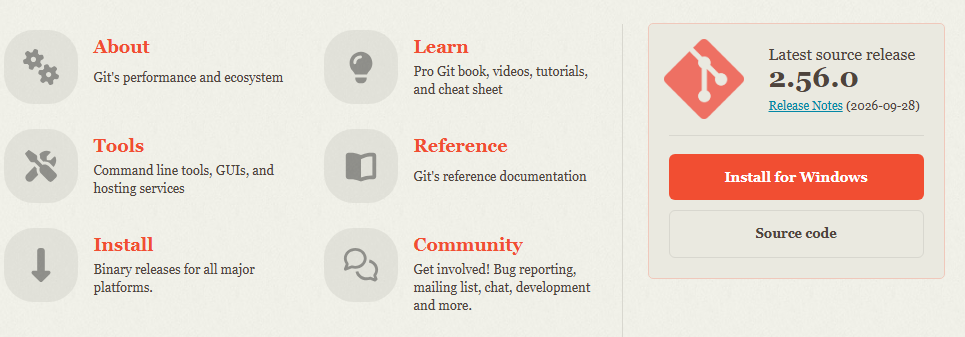
\includegraphics[width=0.807\textwidth,keepaspectratio]{images/1-1.png}
\end{frame}

\begin{frame}{如何安装Git}
	\begin{block}{下载安装包}
		我们能找到很多安装选项：
	\end{block}
	\centering
	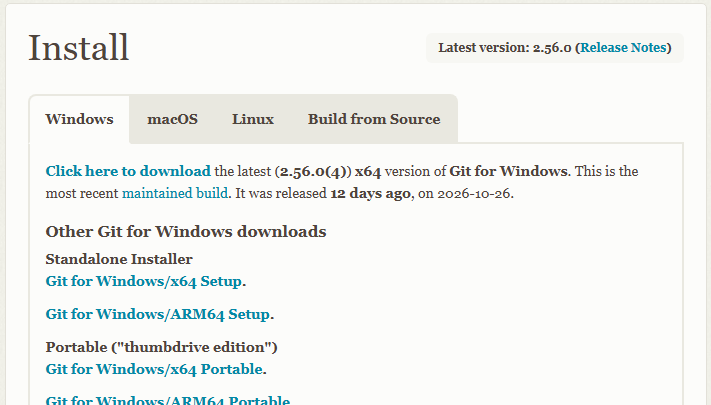
\includegraphics[width=0.61\textwidth,keepaspectratio]{images/1-2.png}
\end{frame}

\begin{frame}{如何安装Git}
\centering
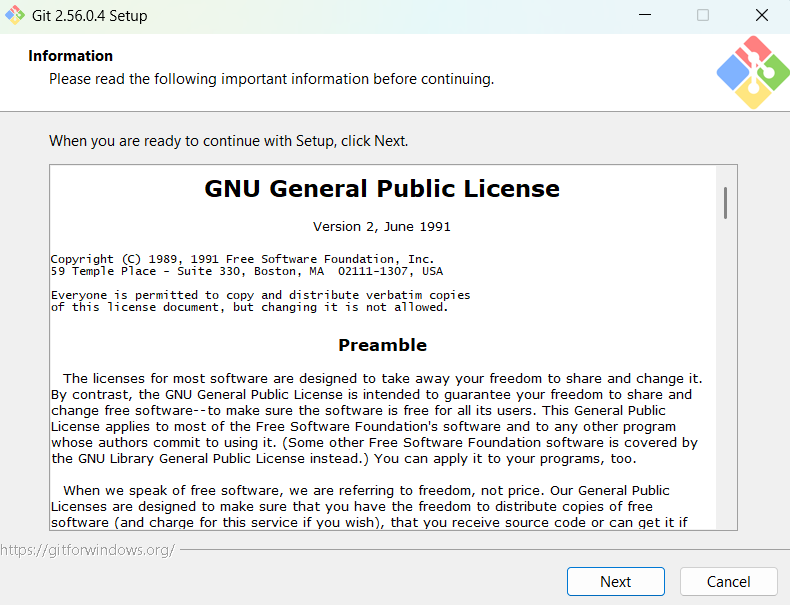
\includegraphics[width=0.61\textwidth,keepaspectratio]{images/1-3.png}
\end{frame}

\begin{frame}{如何安装Git}
	\centering
	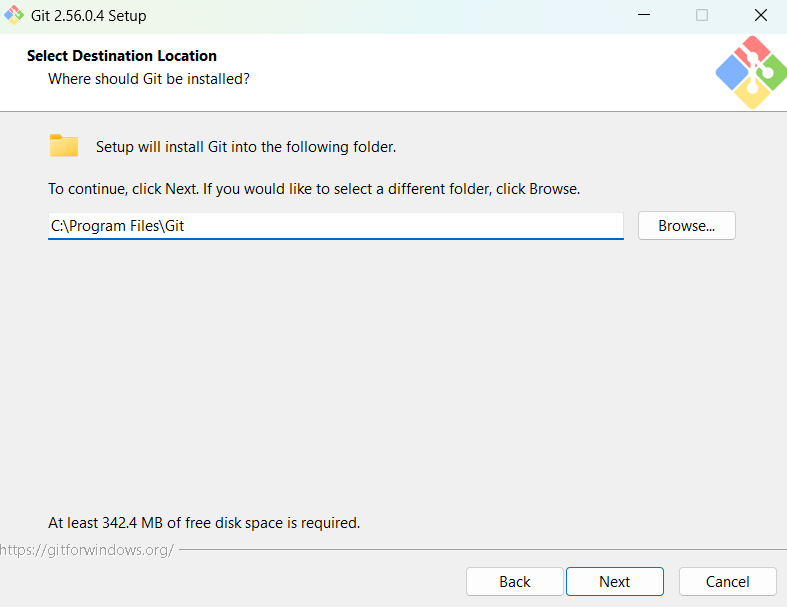
\includegraphics[width=0.61\textwidth,keepaspectratio]{images/1-4.png}
\end{frame}

\begin{frame}{如何安装Git}
	\centering
	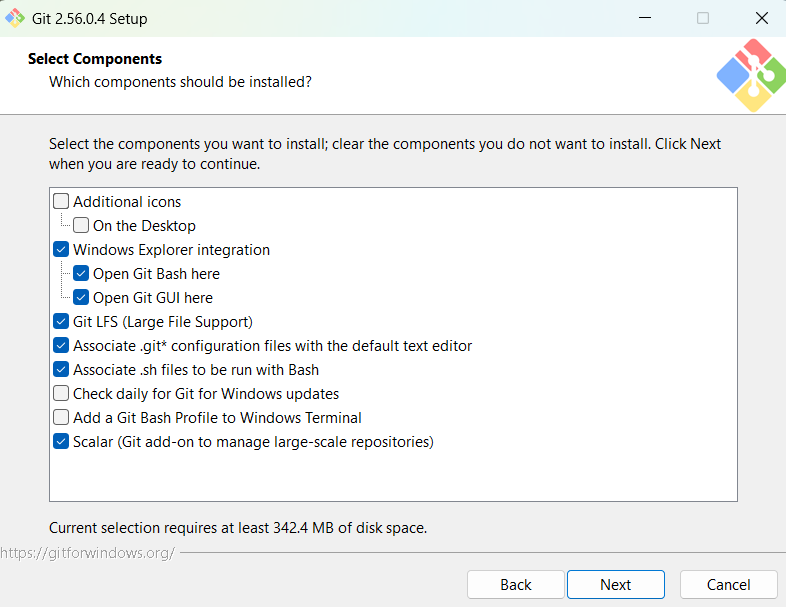
\includegraphics[width=0.58\textwidth,keepaspectratio]{images/1-5-1.png}
	
	这张图片会和现场演示稍有不同，以现场演示为准。
\end{frame}

\begin{frame}{如何安装Git}
	\centering
	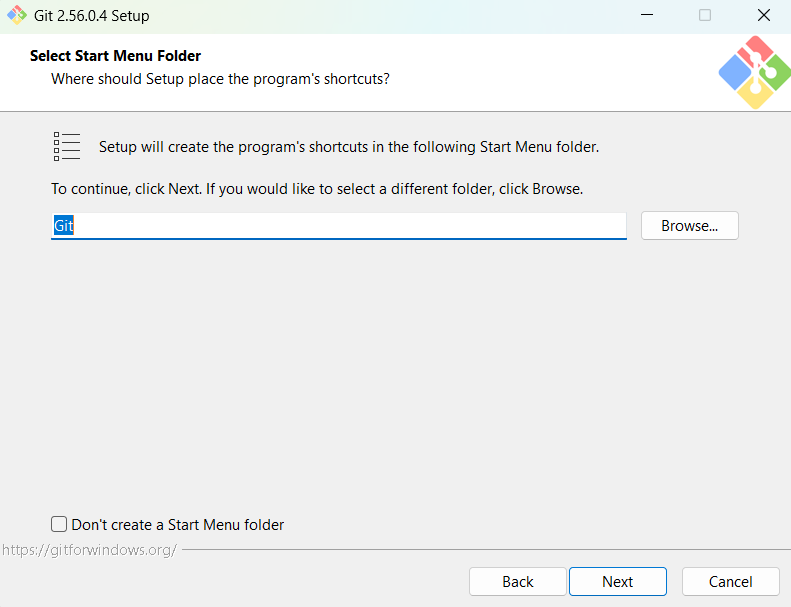
\includegraphics[width=0.61\textwidth,keepaspectratio]{images/1-6.png}
\end{frame}

\begin{frame}{如何安装Git}
	\centering
	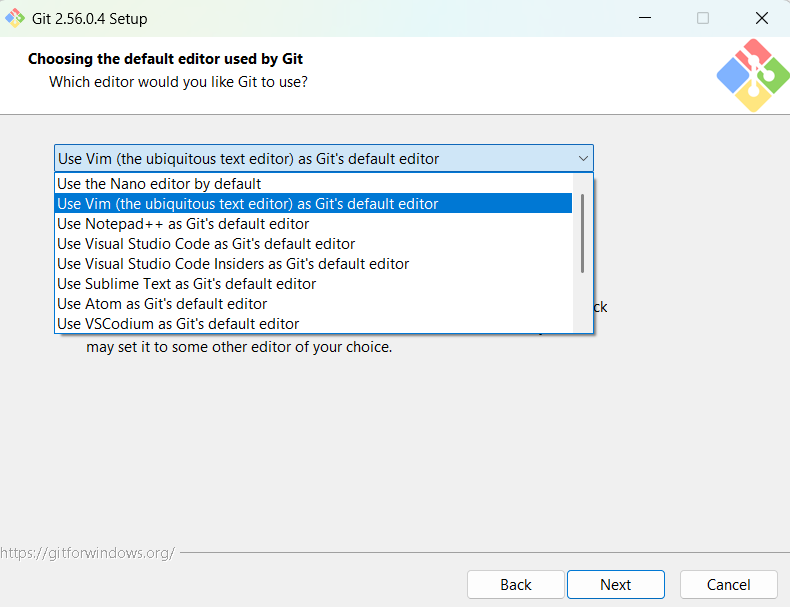
\includegraphics[width=0.58\textwidth,keepaspectratio]{images/1-7.png}
	
	这张图片会和现场演示稍有不同，以现场演示为准。
\end{frame}

\begin{frame}{如何安装Git}
	\centering
	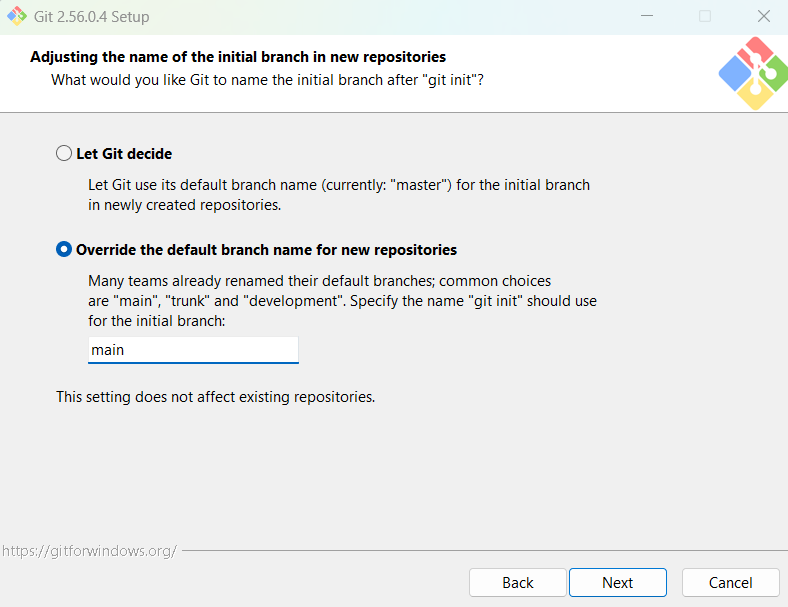
\includegraphics[width=0.61\textwidth,keepaspectratio]{images/1-8.png}
\end{frame}

\begin{frame}{如何安装Git}
	\centering
	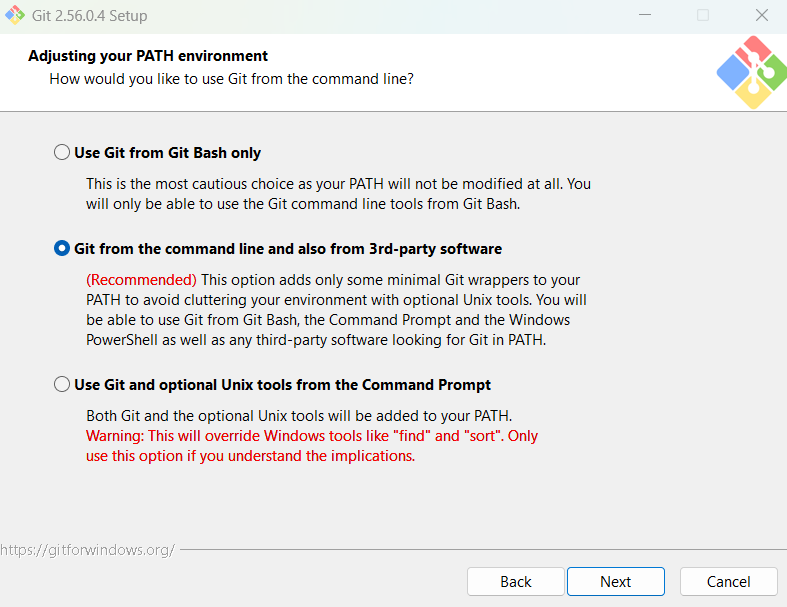
\includegraphics[width=0.61\textwidth,keepaspectratio]{images/1-9.png}
\end{frame}

\begin{frame}{如何安装Git}
	\centering
	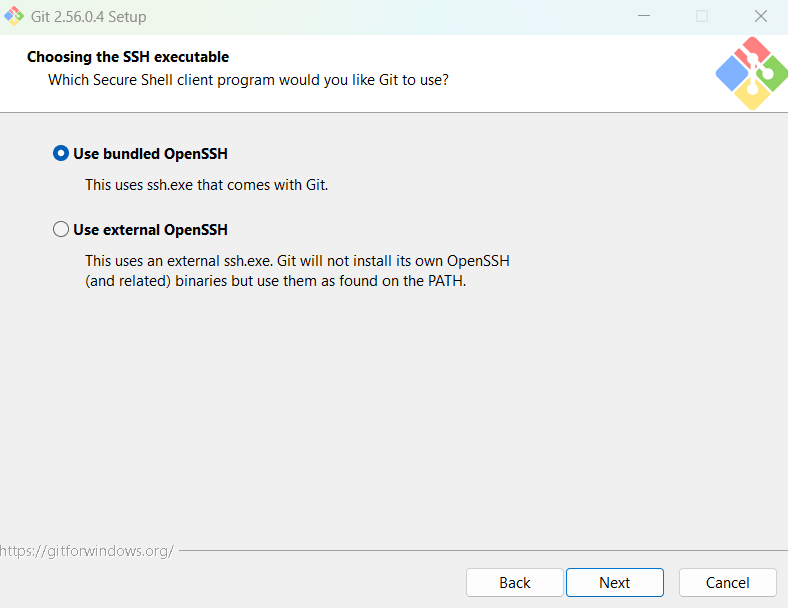
\includegraphics[width=0.61\textwidth,keepaspectratio]{images/1-10.png}
\end{frame}

\begin{frame}{如何安装Git}
	\centering
	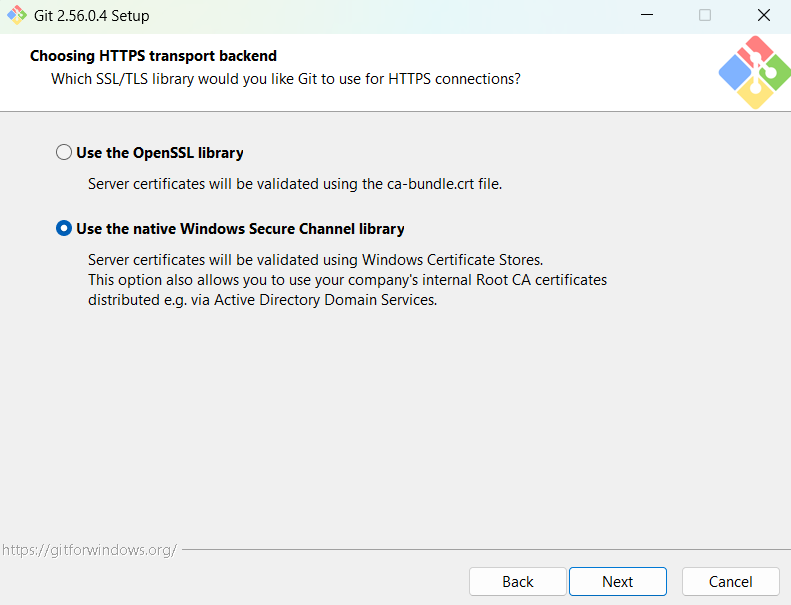
\includegraphics[width=0.61\textwidth,keepaspectratio]{images/1-11.png}
\end{frame}

\begin{frame}{如何安装Git}
	\centering
	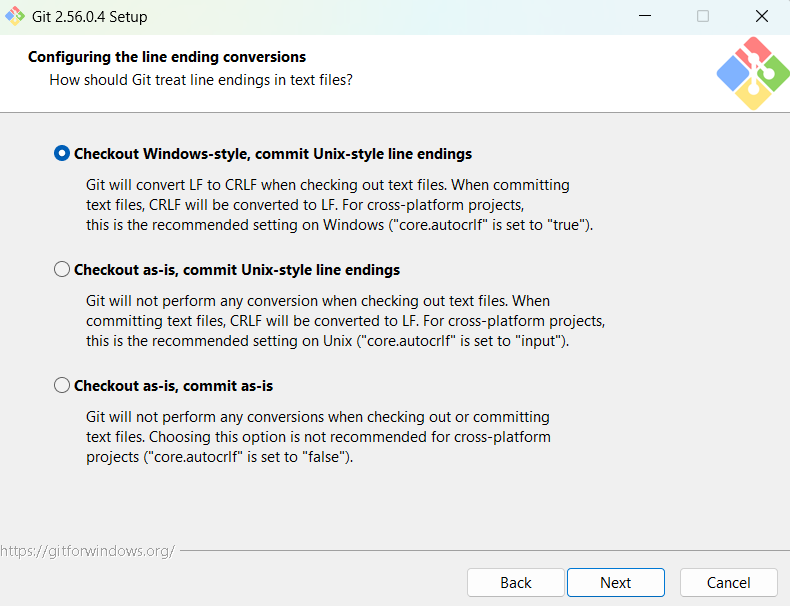
\includegraphics[width=0.61\textwidth,keepaspectratio]{images/1-12.png}
\end{frame}

\begin{frame}{如何安装Git}
	\centering
	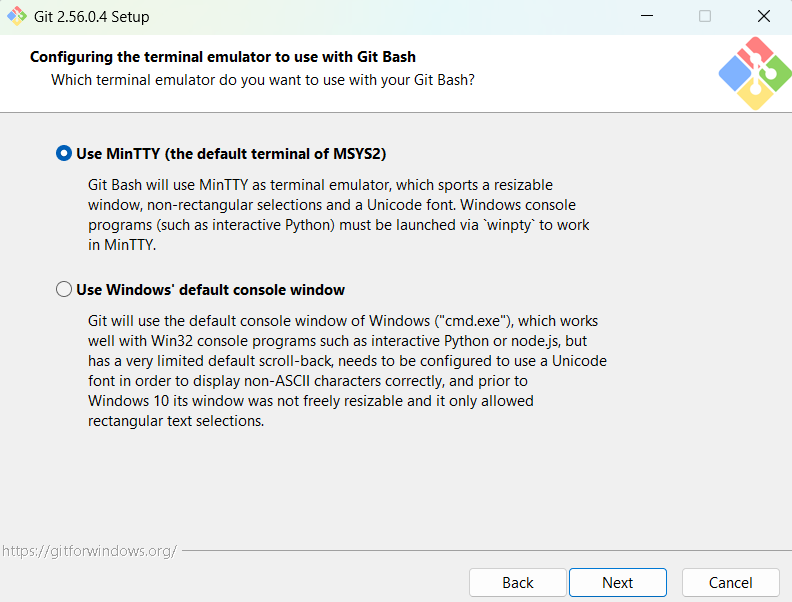
\includegraphics[width=0.61\textwidth,keepaspectratio]{images/1-13.png}
\end{frame}

\begin{frame}{如何安装Git}
	\centering
	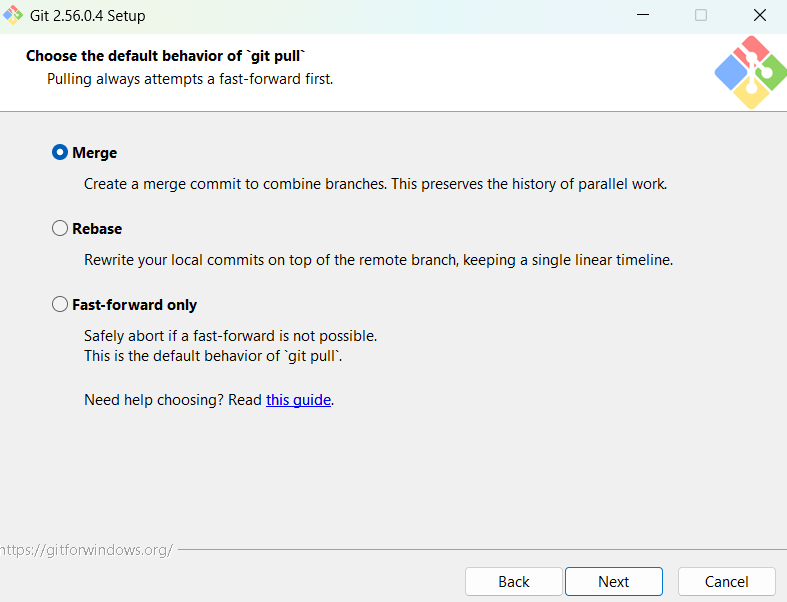
\includegraphics[width=0.61\textwidth,keepaspectratio]{images/1-14.png}
\end{frame}

\begin{frame}{如何安装Git}
	\centering
	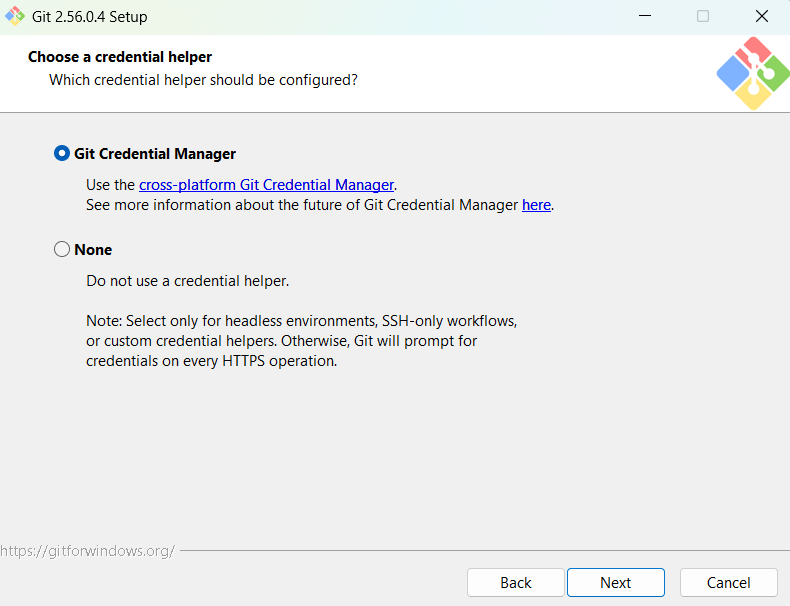
\includegraphics[width=0.61\textwidth,keepaspectratio]{images/1-15.png}
\end{frame}

\begin{frame}{如何安装Git}
	\centering
	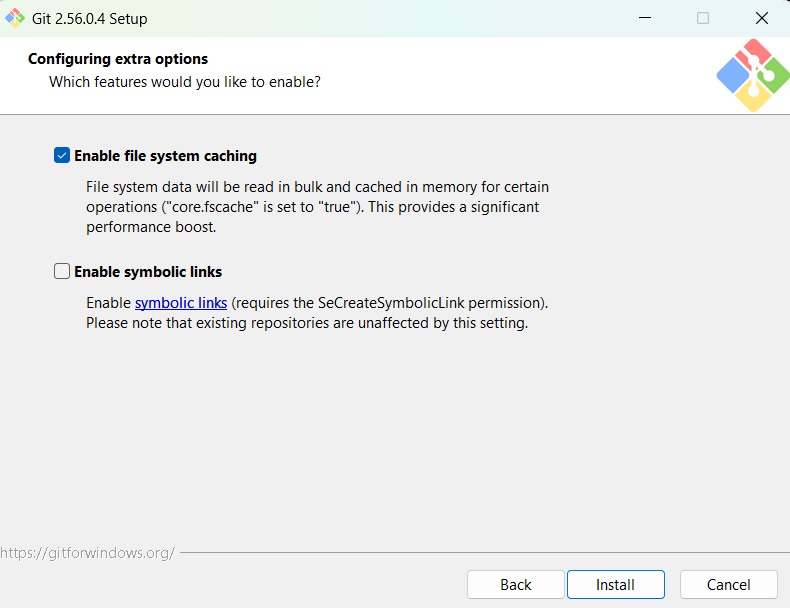
\includegraphics[width=0.61\textwidth,keepaspectratio]{images/1-16.png}
\end{frame}

\begin{frame}{如何安装Git}
	\centering
	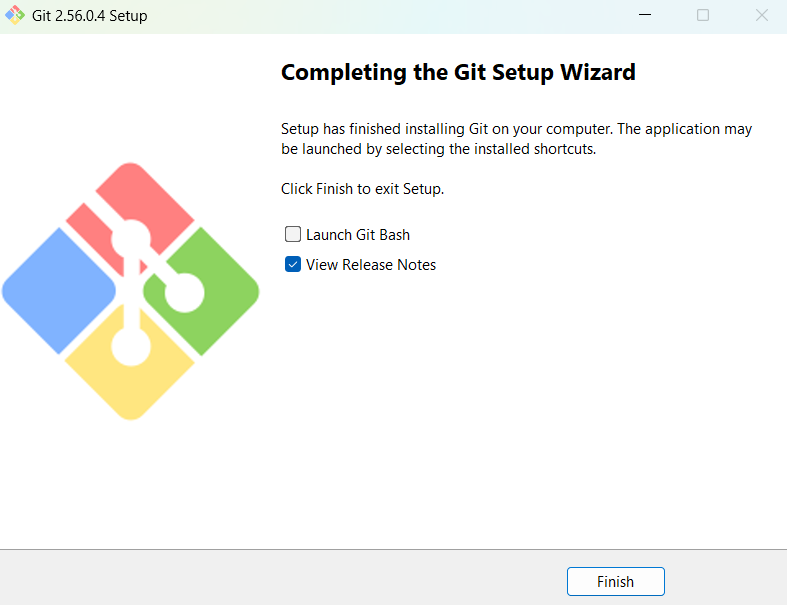
\includegraphics[width=0.58\textwidth,keepaspectratio]{images/1-17.png}
	
	这张图片会和现场演示稍有不同，以现场演示为准。
\end{frame}

\begin{frame}{Git安装成功}
	\begin{block}{安装成功}
		使用 git -{}-version 命令来判断是否安装成功
	\end{block}
	\centering
	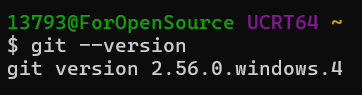
\includegraphics[width=0.35\textwidth,keepaspectratio]{images/2-1.png}
\end{frame}

\begin{frame}{Git配置}
	\begin{block}{配置用户名和邮箱}
		使用如下命令来进行配置
		\begin{itemize}
			\item git config -{}-global user.name “你的用户名”
			\item git config -{}-global user.email “你的邮箱”
		\end{itemize}
	\end{block}
	\centering
	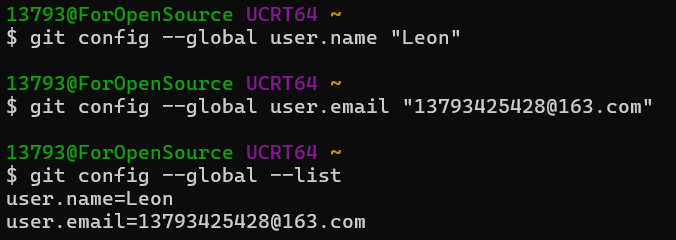
\includegraphics[width=0.61\textwidth,keepaspectratio]{images/2-2.png}
\end{frame}

\begin{frame}{Git 的基本工作原理}
\begin{block}{仓库}
	\hspace*{2em}当我们在一个项目文件夹中执行 `git init` 命令时，Git 会在该文件夹下创建一个名为 `.git` 的隐藏目录，用于保存版本控制所需的信息。此时，该文件夹就成为了一个 Git 仓库。
	
	\hspace*{2em}需要注意的是，Git 并不要求初始化的文件夹必须为空，原有文件也不会受到影响。
\end{block}
	\centering
	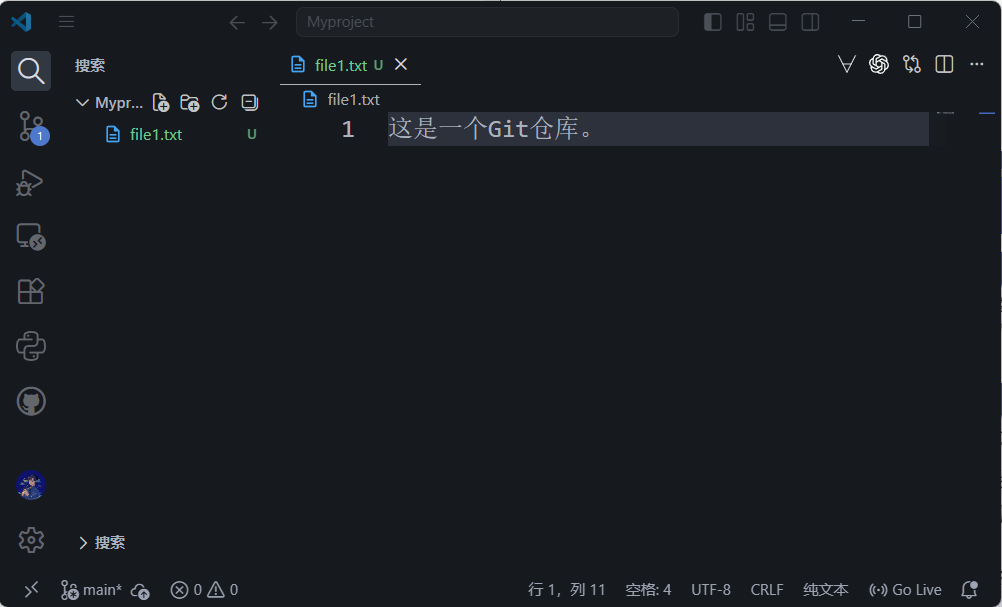
\includegraphics[width=0.507\textwidth,keepaspectratio]{images/3-1.png}
\end{frame}

\begin{frame}{Git 的基本工作原理}
	\begin{block}{.git文件夹}
		\hspace*{2em}这个文件夹在被初始化为仓库之后，就会增加一个名为.git的隐藏文件夹，其中会含有版本控制的重要信息。
	\end{block}
	\centering
	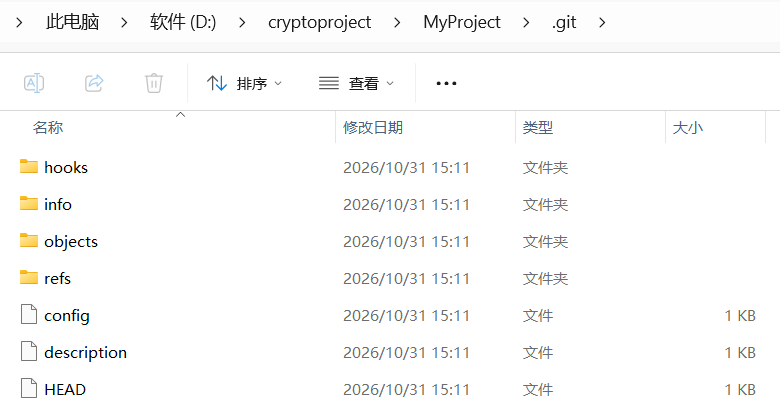
\includegraphics[width=0.507\textwidth,keepaspectratio]{images/3-2.png}
\end{frame}	

\begin{frame}{Git 的基本工作原理}
\begin{block}{工作区}
	\hspace*{2em}我们实际看到和编辑的项目文件。对文件进行修改、创建和删除，都是在这里完成的。
\end{block}
	\centering
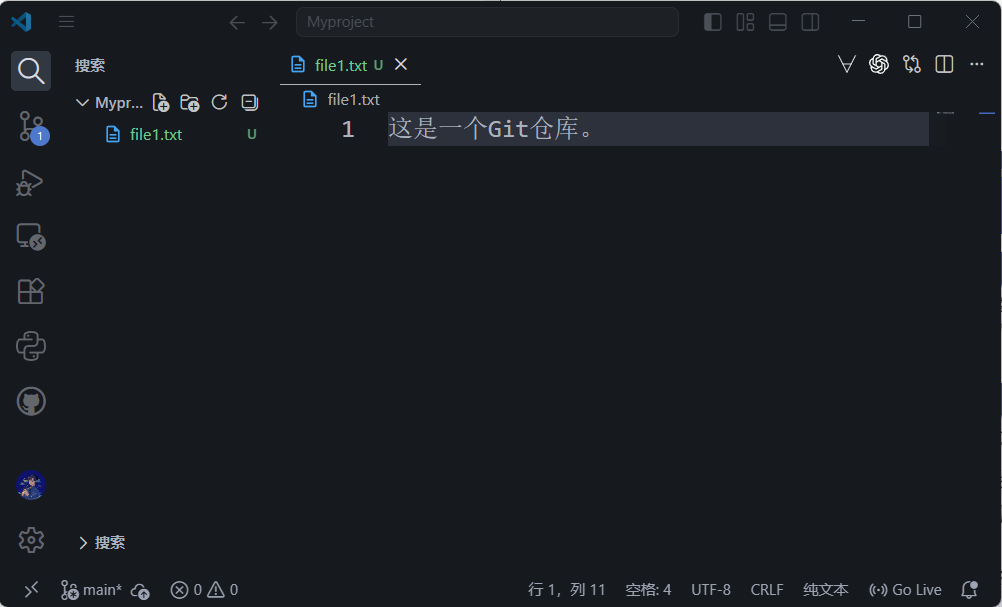
\includegraphics[width=0.64\textwidth,keepaspectratio]{images/3-1.png}
\end{frame}
\begin{frame}{Git 的基本工作原理}
\begin{block}{暂存区}
	\hspace*{2em}我们使用 git add 命令，将指定文件的新增、修改或删除等变化加入暂存区。暂存区并不是一个需要我们手动管理的普通文件夹，其状态信息主要记录在 .git/index 文件中。
\end{block}
\centering
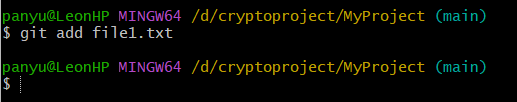
\includegraphics[width=0.707\textwidth,keepaspectratio]{images/3-3.png}	
\end{frame}
\begin{frame}{Git 的基本工作原理}
\begin{block}{版本库}
	\hspace*{2em}当我们执行 git commit 命令时，Git 会根据暂存区中的内容创建一次新的提交（Commit），记录项目在该时刻的状态，并将相应的版本信息保存在 .git 目录中。
	
	\hspace*{2em}每一次提交都有一个唯一的标识符，我们可以使用 git log 命令查看过去的提交记录。
\end{block}
\centering
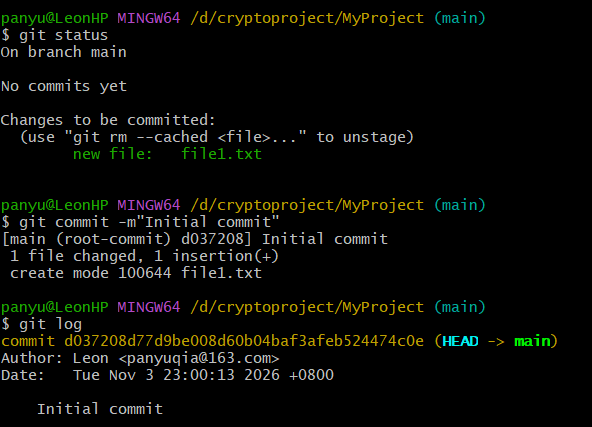
\includegraphics[width=0.407\textwidth,keepaspectratio]{images/3-4.png}
\end{frame}
\begin{frame}{Git 的基本工作原理}
	\centering
	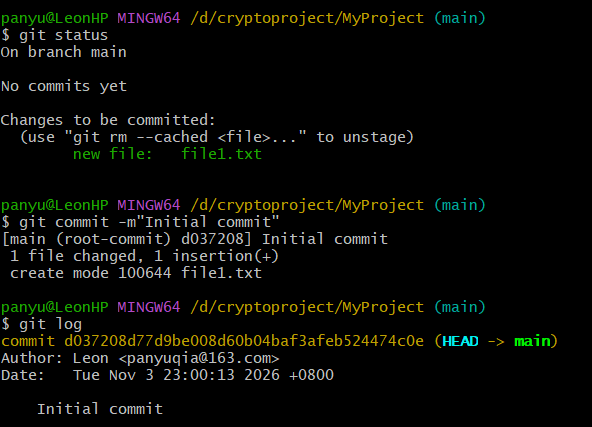
\includegraphics[width=0.61\textwidth,keepaspectratio]{images/3-4.png}
	
	当PYQ看到这一页PPT时就该开始现场演示了。
\end{frame}
\begin{frame}{Git 的基本操作}
	\begin{block}{常用的几条命令}
		\begin{itemize}
			\item git status：查看当前工作区与暂存区的状态
			\item git add 文件名：把指定文件的变化加入暂存区
			\item git commit -m “提交说明”：把暂存区的内容记录为一次提交
			\item git log：查看过去的提交记录
		\end{itemize}
	\end{block}
	
	\begin{block}{Git还有哪些命令呢？}
		\hspace*{2em}其实Git的命令有很多很多，但是由于图形化界面以及Github的存在，不需要掌握那么多的命令。等到大家在某些特定场景下有相关需求时，自己搜索或者问AI就会很快得到答案。等到大家真的面临大且复杂的项目时，大家的能力已经完全足够掌握Git了。
	\end{block}

\end{frame}
\begin{frame}{git status命令}
\begin{block}{git status命令}
	\hspace*{2em}该命令用于查看当前工作区与暂存区的状态，比如当你在工作区新增了一个文件file2.txt时，此时执行该命令你会发现Untracked files字样，表示这是一个新文件，也就是说git还没开始跟踪这个文件。
\end{block}
\centering
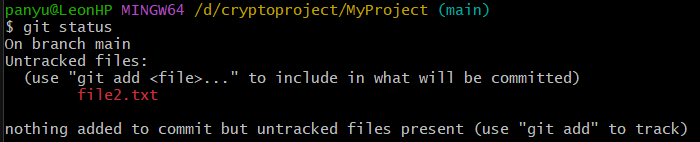
\includegraphics[width=0.707\textwidth,keepaspectratio]{images/4-1.png}
\end{frame}
\begin{frame}{git status命令}
	\begin{block}{git status}
		\hspace*{2em}若你在工作区对原先就存在并且提交过的file1.txt进行了一些修改，此时执行该命令你会发现Changes not staged for commit字样，表示这个修改还没有加入暂存区
	\end{block}
	\centering
	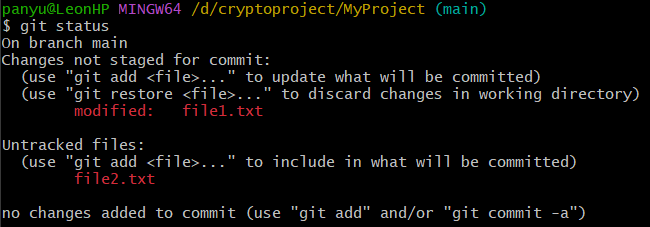
\includegraphics[width=0.707\textwidth,keepaspectratio]{images/4-2.png}
\end{frame}
\begin{frame}{git status命令}
	\begin{block}{git status}
		\hspace*{2em}若你对刚才的两个文件使用过git add之后再使用该命令，此时你会发现Changes to be committed字样，表示这两个修改等待被提交，也就是git commit。
	\end{block}
	\centering
	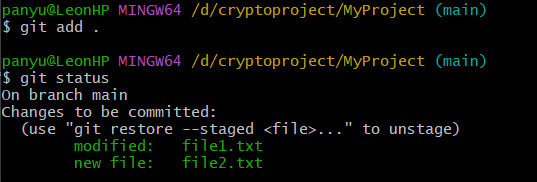
\includegraphics[width=0.707\textwidth,keepaspectratio]{images/4-3.png}
\end{frame}

\begin{frame}[fragile]{git log命令}
	\begin{block}{查看提交历史}
	git log 把提交历史按时间倒序列出来，最新的一次在最上面，一次提交显示成一块。
	\vspace{-0.8em}
{
\begin{semiverbatim}
commit 121e7be060b55a9ed047d1c961323c81a635553f
Author: 潘宇琦 <panyuqi@example.com>
Date:   Wed Nov 25 00:10:18 2026 +0800
    新增 file2.txt
\end{semiverbatim}
		}
	\end{block}
	\begin{block}{每一行是什么}
		\begin{itemize}
			\item commit 后面那串是这次提交的哈希，唯一标识
			\item Author 是作者，Date 是提交时间
			\item 空行下面那一句是提交说明，就是 git commit -m 写的内容
		\end{itemize}
	\end{block}
\end{frame}

\begin{frame}[fragile]{git log命令}
	\begin{block}{git log -{}-oneline}
	执行git log -{}-oneline可以使得每次提交只显示为一行，方便我们查阅。
	\vspace{-0.8em}
		{
\begin{semiverbatim}
121e7be 新增 file2.txt
cd8285d 给 file1.txt 加一行
a4bb704 新增 file1.txt
\end{semiverbatim}
		}
	\end{block}
	\begin{block}{省掉了什么}
		\begin{itemize}
			\item 哈希此时只显示前 7 位，足够我们区分提交。
			\item 作者、时间、空行此时都不会显示。
		\end{itemize}
	\end{block}
\end{frame}

\begin{frame}{git log命令}
	\begin{block}{进入分页器}
		\hspace*{2em}提交数量较多时，git log 不会输出全部提交记录，而是进入分页显示，屏幕最下方会出现一个冒号。
	\end{block}
	\begin{block}{相关操作}
		\begin{itemize}
			\item 按空格或者 PageDown 翻下一页
			\item 按上下方向键一行一行看
			\item 按 q 退出，回到命令行
		\end{itemize}
	\end{block}
\end{frame}

\begin{frame}[fragile]{修改上一次提交}
	\begin{block}{git commit -{}-amend}
		\hspace*{2em}刚提交完时如果发现漏了文件，或者提交说明写错了，可以用它把这次的改动直接补进上一次的提交，同时不会多出一条提交记录。
	\end{block}
\begin{block}{如果漏掉了文件}
{
\begin{semiverbatim}
git add notes.txt      # 先把漏掉的文件加入暂存区
git commit --amend     # 再执行，替换上一次提交(这样写会打开文本编辑器)
\end{semiverbatim}
}
\end{block}
\begin{block}{如果只是写错了说明}
{
\begin{semiverbatim}
git commit --amend -m "新的提交说明"
\end{semiverbatim}
}
\end{block}

\begin{block}{但是}
	amend只能改动最近的一次提交，并且会使哈希值发生变化。我们后面会讲到该命令最好在本地使用。
\end{block}
\end{frame}

\begin{frame}[fragile]{git restore命令}
\begin{block}{两条最常用的撤回命令}
{
\begin{semiverbatim}
git restore notes.txt
git restore --staged notes.txt
\end{semiverbatim}
}
\end{block}
	\begin{block}{它们分别做什么}
		\begin{itemize}
			\item git restore 文件名：丢弃工作区里还没 add 的修改
			\item git restore -{}-staged 文件名：把文件移出暂存区，改动本身还在
			\item 这两条都只作用于尚未提交的内容，已经提交的要另外处理
		\end{itemize}
	\end{block}
	
\end{frame}

\begin{frame}[fragile]{git reset命令}
\begin{block}{git reset}
把当前分支退回到指定的某一次提交。指定哪一次都可以，不限于上一次。
{
\begin{semiverbatim}
git reset --hard 9c1b2ab    # 用提交哈希指定退回到哪一次
git reset --hard HEAD~3     # 往前退 3 次
\end{semiverbatim}
}
\end{block}
	\begin{block}{该命令的三种模式}
		\begin{itemize}
			\item -{}-soft：退回到某次提交，回退的所有改动全部留在暂存区
			\item -{}-mixed：退回到某次提交，回退的所有改动全部留在工作区，默认模式
			\item -{}-hard：退回到某次提交，回退的所有改动全部删掉
		\end{itemize}
	\end{block}
\end{frame}

\begin{frame}[fragile]{.gitignore文件}
\begin{block}{有些文件需要被忽略}
\hspace*{2em}有的时候我们不要求所有的文件都要在仓库里，就比如编译产生的日志记录或者一些临时的文件，根本没有保存它们的必要，这时候就要用到.gitignore文件，被记录在里面的文件会被Git忽略，根本不会被git add等命令注意。
{
\begin{semiverbatim}
# 井号开头是注释，整行被忽略
*.log            # 所有以 .log 结尾的文件（任意目录下）
build/           # 整个 build 目录及其中的内容
/todo.txt        # 只忽略仓库根目录下的 todo.txt，子目录里的不管
!important.log   # 感叹号表示例外：上面的规则不适用于它
\end{semiverbatim}
}
\end{block}

	\begin{block}{但是}
	如果文件已经被提交过，此时再写进.gitignore 并不会把它移出仓库，只能单独删掉再提交。
	\end{block}
\end{frame}

\begin{frame}[fragile]{什么是分支}
	\begin{block}{从某一次提交上另起一条线}
\begin{semiverbatim}
A --- B --- C                main
A --- B --- C --- D --- E    xxxx
\end{semiverbatim}
		在 C 这个提交上建一条分支xxxx，会使得之后的提交只记录在xxxx分支上而不记录在main分支上，main分支仍然停在提交C。
	\end{block}
	\begin{block}{切到不同分支}
		\begin{itemize}
			\item 切到 xxxx：文件是提交A、B、C、D 一路改下来的结果
			\item 切回 main：文件变回提交C之后的样子，后面的所有提交都不会显示
			\item 两条线上的提交互不干扰
		\end{itemize}
	\end{block}
\end{frame}

\begin{frame}{为什么需要分支}
	\begin{block}{一个常见的情况}
		\hspace*{2em}主分支上的代码是能跑的，现在我们要加一个新功能。但是功能写到一半时代码肯定是残缺的，此时既不能提交到主干，又不能把写了一半的部分丢掉。
	\end{block}
	\begin{block}{所以此时需要新开一条支线}
		\begin{itemize}
			\item 主干照旧可用，不影响别人
			\item 新功能在另一条线上写，随便提交
			\item 写完了合并回主干，写废了直接丢掉
		\end{itemize}
	\end{block}
\end{frame}

\begin{frame}[fragile]{分支是一个指针}
	\begin{block}{不是复制文件}
		\hspace*{2em}新建一个分支，并不会把文件复制一份。分支只是一个指向某次提交的指针，所以创建分支几乎不占空间，也非常快。
	\end{block}
	\begin{block}{当前在哪条分支}
		\hspace*{2em}Git 用 HEAD 记录当前所在的分支。切换分支，就是让 HEAD 指向另一个指针，工作区里的文件也会跟着变成那条分支上的样子。
	\end{block}
\end{frame}

\begin{frame}[fragile]{创建与切换分支}
	\begin{block}{常用命令}
{
\begin{semiverbatim}
git branch                # 列出所有分支，当前分支前面有 *
git switch -c xxx         # 新建 xxx 分支并切换过去
git switch main           # 切回 main
git branch -d xxx         # 删除xxx分支
\end{semiverbatim}
}
\end{block}
\end{frame}

\begin{frame}[fragile]{合并分支}
	\begin{block}{git merge}
		先切换回要接收改动的那条分支，再把另一条分支合并进来。
		\vspace{-0.8em}
\begin{semiverbatim}
git switch main
git merge xxxx
\end{semiverbatim}
	\end{block}
	\begin{block}{两种结果}
		\begin{itemize}
			\item 快进：主干没有新提交，直接挪到 xxxx 的最新提交上
			\item 合并提交：两条线都往前走过了，Git 生成一个新的提交把它们接起来
		\end{itemize}
	\end{block}
\end{frame}

\begin{frame}[fragile]{两种合并结果长什么样}
	\begin{block}{快进：只挪指针，不产生新提交}
		{
			\begin{semiverbatim}
before main   A --- B --- C
before xxxx   A --- B --- C --- D --- E
after  main   A --- B --- C --- D --- E
after  xxxx   A --- B --- C --- D --- E
\end{semiverbatim}
		}
	\end{block}
	\begin{block}{合并提交：两条线各走了几步，新建一个提交接起来}
		{
			\begin{semiverbatim}
before main   A --- B --- C --- F
before xxxx   A --- B --- C --- D --- E
after  main   A --- B --- C --- F --- M
after  xxxx   A --- B --- C --- D --- E
\end{semiverbatim}
		}
	\end{block}
\end{frame}

\begin{frame}[fragile]{解决冲突}
	\begin{block}{什么时候会冲突}
		两条分支改了同一个文件的同一处，Git 不知道听谁的，就会停下来让你决定。
		\vspace{-0.8em}
\begin{semiverbatim}
<<<<<<< HEAD
主线上写的内容
=======
分支上写的内容
>>>>>>> xxxx
\end{semiverbatim}
	\end{block}
	\begin{block}{解决步骤}
		\begin{itemize}
			\item 把内容改成最终想要的样子，删掉这三行标记
			\item git add 标记冲突已解决
			\item git commit 完成这次合并
		\end{itemize}
	\end{block}
\end{frame}

\begin{frame}{GitHub 是什么}
	\begin{block}{Git 和 GitHub 不是一回事}
		\begin{itemize}
			\item Git：装在你电脑上的版本控制工具，负责记录提交历史
			\item GitHub：把这些仓库放到网上的平台，负责托管和协作
		\end{itemize}
	\end{block}
	\begin{block}{它能做什么}
		\hspace*{2em}把本地仓库放到互联网上，让别人也能看到、下载、提意见，甚至直接帮你修改。没有 GitHub，Git 一样能用，但只能在你自己电脑上。
	\end{block}
\end{frame}

\begin{frame}{GitHub 的意义}
	\begin{block}{它不只是一个放代码的网站}
		\begin{itemize}
			\item 找资源：想找某个库、想学某个功能怎么实现，第一站就是这里
			\item 有流程：Issue 讨论、PR 看改动、Review 逐行提意见，都在一个页面里
			\item 门槛低：不用谁给权限，fork 一份就能改
			\item 有记录：提交和 PR 都挂在账号下，谁都能看到
			\item 联系其他开发者：在 Issue 里能直接跟作者和维护者对话
		\end{itemize}
	\end{block}
	\begin{block}{本课程的仓库}
https://github.com/Leon5428/ThisIsOpenSource

课件、讲义都在这个仓库里，可以给作者点点star。
\end{block}
\end{frame}

\begin{frame}{新建一个仓库}
	\begin{block}{在网页上操作}
		\hspace*{2em}登录 GitHub，点右上角的加号，选择 New repository，填一个仓库名，选择公开或者私有，然后点 Create repository。
	\end{block}
\centering
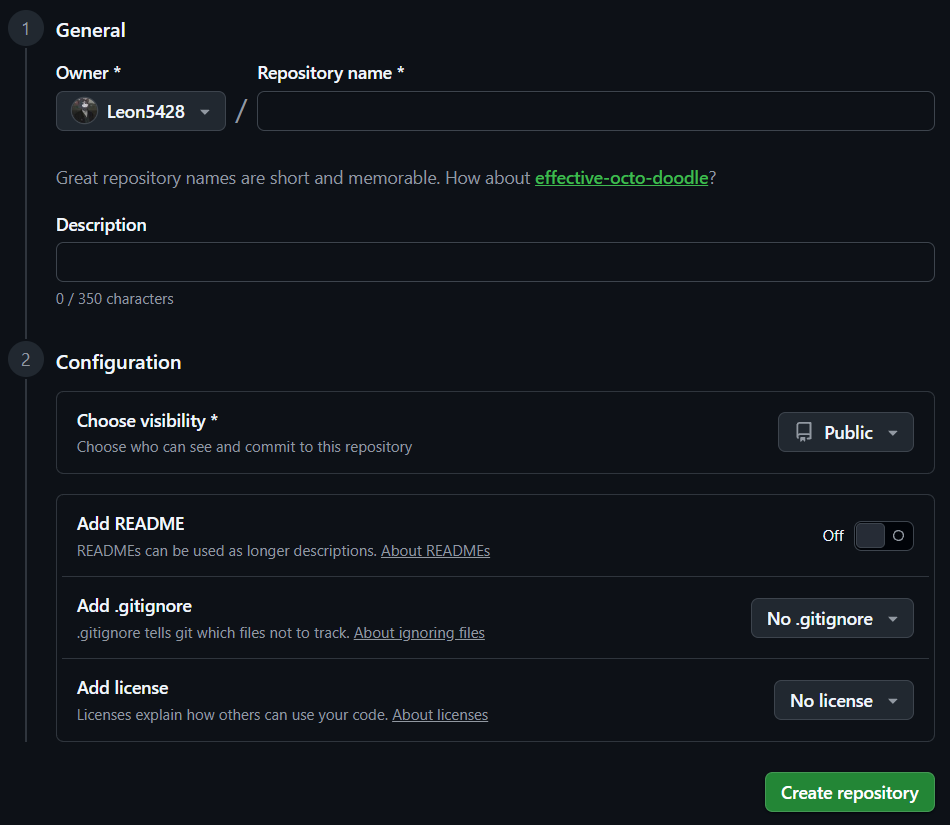
\includegraphics[width=0.407\textwidth,keepaspectratio]{images/5-1.png}
\end{frame}

\begin{frame}[fragile]{克隆到本地}
\begin{block}{git clone}
把远程仓库完整下载到本地，并自动把这个远程地址记成 origin。
\vspace{-0.8em}
\begin{semiverbatim}
git clone https://github.com/你的用户名/仓库名.git
\end{semiverbatim}
\end{block}
	\begin{block}{clone 和 init 的区别}
		\begin{itemize}
			\item git init：从零开始建一个空仓库
			\item git clone：把远程已有的仓库连历史一起拿下来
		\end{itemize}
		clone 下来的仓库不用再执行 git init 了，因为它已经是一个完整的仓库了。
	\end{block}
\end{frame}

\begin{frame}[fragile]{把本地提交推上去}
\begin{block}{git push}
本地 commit 之后，历史只存在你的电脑上。push 把它送到远程仓库。
\vspace{-0.8em}
\begin{semiverbatim}
git add 文件名
git commit -m "提交说明"
git push -u origin main    # 第一次推送(git init才需要这条命令)
git push                   # 之后直接这样
\end{semiverbatim}
\end{block}
\begin{block}{-u 做了什么}
\hspace*{2em}把本地的 main 和远程的 origin/main 关联起来，之后 git push、git pull 都不用再写后面那一串。
\end{block}
\end{frame}

\begin{frame}[fragile]{git push 到底有多少参数}
\begin{block}{官方文档里的全部选项}
{
\begin{semiverbatim}
-v --verbose          -q --quiet          -n --dry-run
-f --force            --force-with-lease  --force-if-includes
--all --branches      --mirror            --prune
-d --delete           --tags              --follow-tags
-u --set-upstream     --atomic            --no-atomic
--recurse-submodules  --thin              --no-thin
--porcelain           --progress          --no-verify
--verify              -o --push-option    --signed
--no-signed           --receive-pack      --exec
--repo                -4 --ipv4           -6 --ipv6
\end{semiverbatim}
}
\end{block}

\end{frame}

\begin{frame}[fragile]{远程仓库也有分支}
	\begin{block}{本地看到的只是副本}
		\hspace*{2em}远程仓库里除了 main，还可能有别的分支。clone 只把默认分支检出成工作区，但每一个远程分支都在本地留了一个只读的副本，名字前面带 origin/。
\begin{semiverbatim}
git branch -r      # 只看远程分支：origin/main、origin/xxxx
git branch -a      # 本地和远程的一起列出
\end{semiverbatim}
	\end{block}
	\begin{block}{不能直接改 origin/xxxx}
		\hspace*{2em}它们是引用，不是能提交的分支。要改，先在本地建一个对应的分支。
	\end{block}
\end{frame}

\begin{frame}[fragile]{本地分支\&远程分支}
\begin{block}{情况一：本地有，远程没有}
我们在本地建立完一个 xxxx 分支之后，远程最开始是不知道的，所以需要在第一次推送的时候把远程分支建出来。
\begin{semiverbatim}
git push -u origin xxxx    # 推到 origin，并在远程建出同名的xxxx分支
\end{semiverbatim}
加了 -u 会绑定远程的相对应的xxxx分支，以后再提交直接 git push 就行；不加的话，以后敲 git push 会报 fatal: no upstream branch。
\end{block}
\begin{block}{情况二：clone时远程有，本地没有}
此时本地只有 origin/xxxx 这个分支的快照，只需要切一下就会建出对应的本地分支。
\begin{semiverbatim}
git switch xxxx           # 自动建本地xxxx分支，跟踪 origin/xxxx
\end{semiverbatim}
\end{block}
\end{frame}

\begin{frame}[fragile]{本地分支\&远程分支}
\begin{block}{情况三：clone时远程没有xxx分支，克隆后在远程建立了xxx分支}
\hspace*{2em}此时我们先需要git fetch，该命令把远程各个分支的新提交下载到本地的 origin/*，并且只更新这些副本，不改动工作区，也不会切换分支。完成git fetch之后再进行git switch。
\begin{semiverbatim}
git switch xxxx
\end{semiverbatim}
它用的是本地已经存在的 origin/xxxx，不会再去远程拿新东西。
\end{block}
\end{frame}

\begin{frame}{个人使用 $\Rightarrow$ 团队合作}
	\begin{block}{如何团队合作}
		\begin{itemize}
			\item 建一个仓库，把组员加成协作者
			\item 按任务开分支：一个功能一条分支，也可以几个人共用一条
			\item 在分支上写、提交，把这条分支推上去
			\item 提 Pull Request，请别人看
			\item 通过之后合并进 main
		\end{itemize}
	\end{block}
	\begin{block}{当我们开始工作时}
		因为clone下来时工作区默认是对应主分支的，所以我们需要先切换到我们负责的分支，再进行后续的工作。
	\end{block}
\end{frame}

\begin{frame}[fragile]{把远程的改动拉下来}
\begin{block}{git pull}
别人推了新提交，我们本地还是旧的，用 pull 把它们取回来并合并到当前分支。
\vspace{-0.8em}
\begin{semiverbatim}
git pull                           #之前执行过git push -u origin xxxx
git pull origin xxxx            #之前从没有执行过git push -u origin xxxx
git branch --set-upstream-to=origin/xxxx
\end{semiverbatim}
\end{block}
	\begin{block}{git fetch}
		\hspace*{2em}它把远程的新提交下载到本地，但是只更新本地保存的对于远程仓库的快照，我们自己的分支和工作区都不会改变。
		\begin{itemize}
			\item 想合：再执行 git merge origin/main
			\item 不想合：什么都不用做，和没下载过一样
		\end{itemize}
	\end{block}
\end{frame}

\begin{frame}{推送被拒绝怎么办}
	\begin{block}{常见情况}
		\hspace*{2em}别人先推了提交，你的本地落后了，Git 会拒绝这次 push，提示 non-fast-forward。
	\end{block}
\begin{block}{处理办法}
	\begin{itemize}
		\item 先 git pull，把远程的提交合并进来；绝大多数情况下它会自动合上
		\item 只有两边改了同一个文件的同一处，才会停下来等手工解决
		\item 冲突解决完，再 git push
	\end{itemize}
\end{block}
\end{frame}

\begin{frame}{用 Pull Request 合并分支}
	\begin{block}{在网页上把 xxxx 分支合并到main分支 }
		\begin{enumerate}
			\item 先把分支推上去：git push -u origin feature（新开的分支第一次推要加 -u）
			\item 仓库首页会出现 Compare \& pull request，点它
			\item 上面选 base 为 main，下面选 compare 为 feature
			\item 填标题和说明，点 Create pull request
			\item 别人看过之后，点 Merge pull request
		\end{enumerate}
	\end{block}
	\begin{center}
		\alert{合并发生在 GitHub 上，我们本地的 main 还要 pull 一次才更新。}
	\end{center}
\end{frame}

\begin{frame}{合并一个 PR 的三种方式}
	\begin{block}{点 Merge 旁边的箭头才看得到}
		\begin{itemize}
			\item Create a merge commit：保留分支上的每一条提交，另加一个合并提交
			\item Squash and merge：把分支上的提交压成一条
			\item Rebase and merge：把提交逐条接到 main 后面，不产生合并提交
		\end{itemize}
	\end{block}
	\begin{block}{合并之后}
		\hspace*{2em}页面会提示 Delete branch，把已经合掉的分支删掉，仓库才不会越堆越乱。
	\end{block}
\end{frame}

\begin{frame}{读懂一个仓库}
	\begin{block}{学习他人仓库}
		\hspace*{2em}Github会有很多优质仓库，如果想知道它是干什么的、能不能用、怎么为这个仓库做贡献，可以先在网页端浏览下面这几个文件。
		\begin{itemize}
			\item README：这个项目是做什么的、怎么安装、怎么用
			\item LICENSE：别人允许你拿它做什么
			\item CONTRIBUTING：想贡献要先遵守什么规矩
			\item 目录结构和最近的提交：项目大概怎么组织的
		\end{itemize}
	\end{block}
\end{frame}

\begin{frame}{常见的几种许可证}
	\begin{block}{看到这些名字要知道意思}
		\begin{itemize}
			\item MIT：最宽松，保留版权声明就可以随便用
			\item Apache 2.0：和 MIT 接近，另外明确给了专利授权
			\item GPLv3：用了它，你的修改也必须开源
		\end{itemize}
	\end{block}
	\begin{block}{没有许可证的仓库}
		\hspace*{2em}没有 LICENSE 文件，默认就是保留所有权利，只能看，不能复制和修改。
	\end{block}
\end{frame}

\begin{frame}{用 Issue 提问题}
	\begin{block}{Issue 是什么}
		\hspace*{2em}仓库里的一个公开讨论区，报错、提需求、问问题都在这里。提之前先搜一下有没有人提过同样的问题。
	\end{block}
	\begin{block}{一个能被回复的 Issue 至少写清}
		\begin{itemize}
			\item 标题：一句话说清是什么问题
			\item 复现步骤：怎么操作才会出现
			\item 期望的结果和实际的结果
			\item 环境：系统、版本号
		\end{itemize}
	\end{block}
\end{frame}

\begin{frame}{Fork}
	\begin{block}{为什么需要 fork}
		\hspace*{2em}别人的仓库你没有写权限，不能直接 push。fork 会把这个仓库复制一份到你的账号下，那一份你可以随便改。
	\end{block}
	\begin{block}{fork 和 clone 的区别}
		\begin{itemize}
			\item fork：发生在 GitHub 上，复制出一个属于你的远程仓库
			\item clone：发生在你电脑上，把某个仓库下载下来
		\end{itemize}
	\end{block}
\end{frame}

\begin{frame}[fragile]{多个远程：upstream}
	\begin{block}{fork 之后本地有两个远程}
		\begin{itemize}
			\item origin：你自己账号下的那一份
			\item upstream：原来的仓库，别人的更新从这里来
		\end{itemize}
	\end{block}
\begin{block}{把原仓库加进来}
\begin{semiverbatim}
git remote add upstream https://github.com/原作者/仓库.git
git remote -v              # 看清两个远程各自的地址
git fetch upstream         # 把原仓库的更新拿下来
git merge upstream/main    # 再合进本地的 main
\end{semiverbatim}
\end{block}
\end{frame}

\begin{frame}{Pull Request：请对方收下你的改动}
	\begin{block}{流程}
		\begin{itemize}
			\item 在你自己的仓库里改好、提交、push
			\item 回到原来的仓库，点 New pull request
			\item 写清改了什么、为什么改
		\end{itemize}
	\end{block}
	\begin{block}{PR 页面能看到什么}
		\hspace*{2em}GitHub 会把你的改动和原仓库逐行对比出来，维护者看的就是这个页面。
	\end{block}
\end{frame}

\begin{frame}{Code Review}
	\begin{block}{维护者会做什么}
		\begin{itemize}
			\item 在具体某一行上留评论
			\item 要求你修改，你改完再 push 到同一个分支即可
			\item 满意之后 approve，然后合并进主分支
		\end{itemize}
	\end{block}
	\begin{center}
		\alert{被指出问题很正常，改完在同一个 PR 里继续讨论。}
	\end{center}
\end{frame}

\begin{frame}{一次完整的协作}
	\begin{block}{从发现问题到被合并}
		\centering
		发现问题
		$\longrightarrow$
		fork
		$\longrightarrow$
		clone
		$\longrightarrow$
		新建分支
		
		提交
		$\longrightarrow$
		push
		$\longrightarrow$
		提 PR
		$\longrightarrow$
		Review
		$\longrightarrow$
		合并
	\end{block}
\end{frame}

\begin{frame}
	\title{谢谢大家}
	\subtitle{第二讲：Git 与 GitHub}
	\author{潘宇琦\hspace*{1em}申鹏威}
	\date{2026年11月}
	\titlepage
\end{frame}

\end{document}